\bookchapter{Capítulo 49: Montando o ambiente de desenvolvimento — Android Studio e o primeiro projeto}

\chapterintro{Para fazer bem o trabalho, é preciso primeiro afiar as ferramentas. Neste capítulo montamos a “cozinha”: instalar o Android Studio, fazer o emulador rodar, criar o primeiro projeto Android da sua vida e desmontar a estrutura do projeto para entender cada peça. Com o ambiente pronto, você verá pela primeira vez o código que escreveu virar um botão clicável — um momento que muita gente guarda a vida inteira.}

\booksection{Instalando o Android Studio}

O Android Studio é o ambiente de desenvolvimento integrado (IDE) oficial do Google, gratuito e do tipo “tudo-em-um”: escrever código, ver a pré-visualização da interface, depurar e gerar o pacote, tudo nele. Quatro passos para instalar:

\begin{enumerate}
  \item Abra o site oficial developer.android.com/studio e baixe a versão estável mais recente (em agosto de 2026, a versão posterior à Narwhal; há versões para Windows/Mac/Linux);
  \item Execute o instalador e vá dando "Avançar" — o assistente já inclui automaticamente o Android SDK e os componentes do emulador;
  \item No primeiro início, baixe os componentes do SDK conforme as instruções (deixe as opções padrão marcadas; pode levar alguns minutos e alguns GB de espaço);
  \item No fim, você verá a tela de boas-vindas — parabéns, a "cozinha" está pronta.
\end{enumerate}

\begin{tcbwarn}{Atenção: tenha os requisitos de hardware na ponta do lápis}
O Android Studio é um “come-memória”: o ideal é partir de 16 GB de RAM (8 GB até rodam, mas o emulador fica travado), reserve mais de 20 GB de disco e use uma CPU com suporte a virtualização (ative VT-x/AMD-V na BIOS). Se o computador for realmente antigo, use a “depuração em aparelho real” no lugar do emulador (falaremos na quarta seção deste capítulo); a experiência sai até mais fluida.

\end{tcbwarn}

\booksection{Criando o seu primeiro projeto}

Na tela de boas-vindas, clique em New Project, escolha o modelo Empty Activity (o mais limpo para iniciantes) e preencha três coisas:

\begin{center}
\begin{tabularx}{\linewidth}{|X|X|X|}
\hline
\textbf{Item de configuração} & \textbf{O que preencher} & \textbf{Descrição} \tabularnewline
\hline
Name & My First App & O nome do app, exibido na tela inicial do celular \tabularnewline
Package name & com.example.myfirstapp & Identificador único no mundo; o costume é "domínio invertido", deixe o padrão por ora \tabularnewline
Minimum SDK & API 26(Android 8.0) & Versão mínima suportada, cobrindo 95\%+ dos aparelhos \tabularnewline
\hline
\end{tabularx}
\end{center}

\begin{center}\small\color{gray}As três coisas a preencher ao criar um projeto\end{center}

Depois de clicar em Finish, o Android Studio usa o Gradle para baixar as dependências e construir o projeto automaticamente (na primeira vez são alguns minutos; depois fica bem mais rápido). Com a build concluída, você já tem um app que roda — embora, por ora, ele só saiba mostrar um “Hello Android!”.

\begin{tcbinfo}{Dica: os segredos do nome de pacote}
O nome de pacote (package name) é como o “número de identidade” do app: não pode repetir no mundo inteiro e não pode mais ser mudado depois da publicação. Para praticar, com.example.xxx serve; em produto formal, troque pelo seu próprio domínio invertido (por exemplo, com.seunome.nome-do-app). Não publique com com.example — a loja recusa o pacote.

\end{tcbinfo}

\booksection{Colocando para rodar: emulador e aparelho real}

Com o código pronto, é preciso encontrar um “celular” para rodá-lo. Você tem duas opções:

\booksubsection{O emulador (Emulator)}

O emulador é um celular Android virtual dentro do computador. No Android Studio, abra Device Manager Create Device, escolha um aparelho (recomendo a linha Pixel) selecione uma imagem de sistema (com Google APIs) baixe inicie. Depois clique no triângulo verde Run, na barra de ferramentas; em alguns segundos, o seu app aparecerá na tela do “celular”.

\booksubsection{Depuração em aparelho real (a mais recomendada)}

O aparelho real é sempre o ambiente de teste mais fiel — o toque ao deslizar, a rede de verdade, os sensores reais; nada disso o emulador reproduz. Depurar num celular Android é simples:

\begin{enumerate}
  \item No celular, abra [Configurações] [Sobre o telefone] e toque 7 vezes seguidas em "Número da versão" para ativar as "Opções do desenvolvedor";
  \item Em [Opções do desenvolvedor], ative a Depuração USB;
  \item Conecte o celular ao computador com o cabo de dados e, no pop-up do celular, escolha "Permitir depuração USB";
  \item Volte ao Android Studio: o seu celular vai aparecer na lista de dispositivos da barra de ferramentas; clique em Run.
\end{enumerate}

\textbf{Alerta de armadilha: não deixe a Depuração USB sempre ativada}\par

A Depuração USB funciona como abrir uma “porta dos fundos” para o computador. Ao carregar em lugares públicos ou conectar a computadores que não são de confiança, desative a Depuração USB sem falta, para evitar que outros leiam os seus dados por ela. No dia a dia, desligue assim que terminar de desenvolver; faça disso um hábito.

\booksection{Desmontando a estrutura do projeto: para que serve cada arquivo}

Ao abrir o projeto pela primeira vez, a árvore de arquivos à esquerda pode deixar você tonto. Calma: no dia a dia, 90\% do seu tempo será com estes poucos itens:

\begin{center}
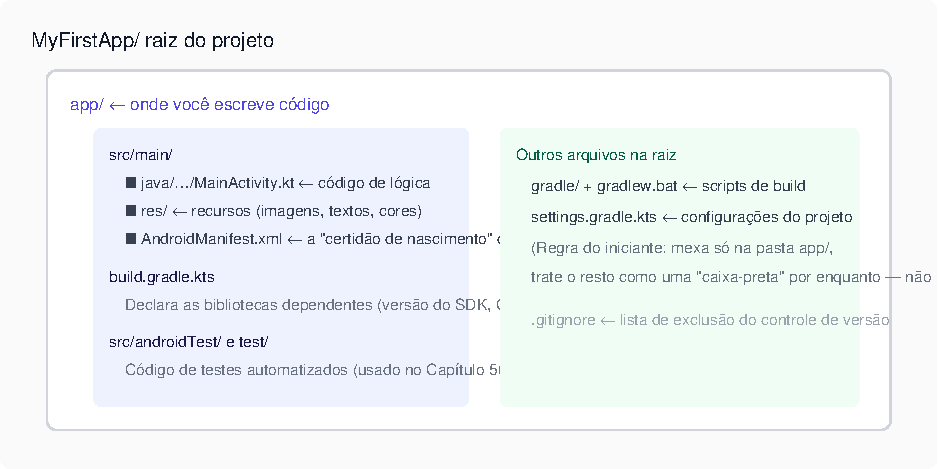
\includegraphics[width=0.92\linewidth]{figures/fig-di-si-shi-jiu-zhang-1}
\\[2pt]\small Figura 2: A estrutura do projeto que todo iniciante precisa entender (regra de bolso: mexa só na pasta app/)
\end{center}

\begin{itemize}
  \item MainActivity.kt: a "porta de entrada" do app. Quando o usuário toca no ícone, é ela a primeira a ser despertada. No modelo atual, ela é a responsável por mostrar "Hello Android!".
  \item AndroidManifest.xml: o "registro de residência" do app — declara como o app se chama, qual é o ícone, quais telas existem e quais permissões ele usa (câmera, localização etc.).
  \item A pasta res/: o depósito de recursos, onde ficam imagens, ícones, textos e cores. Colocar os textos em arquivos de recurso em vez de deixá-los fixos no código é um bom hábito do desenvolvimento Android (facilita trocar idioma e tema).
  \item build.gradle.kts: a "receita" da build — declara a versão mínima suportada e quais bibliotecas são dependências (como o Compose).
\end{itemize}

\booksection{Primeira prova: troque o “Hello” pelo seu nome}

Abra o MainActivity.kt e você verá o código gerado pelo modelo do Compose. Localize a linha Text(“Hello Android!”), troque o texto entre aspas pelo seu nome, por exemplo Text(“Olá, João! Este é o meu primeiro app”), e pressione Ctrl+R (Cmd+R no Mac) para rodar de novo. Em poucos segundos, o seu nome aparece no emulador.

\begin{lstlisting}[language=Kotlin]
setContent {
    MyFirstAppTheme {
        Surface(modifier = Modifier.fillMaxSize()) {
            // v mude isto para o seu texto
            Text("Olá, João! Este é meu primeiro app")
        }
    }
}
\end{lstlisting}

Parabéns: você acabou de completar um ciclo inteiro de “editar o código compilar instalar rodar”. Esse ciclo é a rotina diária de desenvolvimento de agora em diante. Aproveite a empolgação e tente mudar mais coisas: aumente o tamanho da fonte, troque a cor — no próximo capítulo você vai aprender de onde vem essa “mágica”.

\booksection{Primeiros socorros para erros comuns: o “pronto-socorro” das duas primeiras semanas}

Na fase de configuração do ambiente e da primeira build, é bem provável que você esbarre nestes três erros. Sem pânico: todos têm antídoto:

\begin{center}
\begin{tabularx}{\linewidth}{|X|X|X|}
\hline
\textbf{Erro observado} & \textbf{Causa comum} & \textbf{Antídoto} \tabularnewline
\hline
Gradle sync failed / download lento das dependências & Acesso de rede aos repositórios instável & Configure espelhos de repositório para o Gradle (espelhos maven da Alibaba Cloud/Tencent Cloud); pesquise "gradle mirror" na internet e ajuste seguindo o tutorial \tabularnewline
Componentes do SDK faltando & O download do SDK foi pulado na instalação & Em Settings SDK Manager, instale as plataformas e ferramentas que faltam \tabularnewline
O emulador não inicia / tela preta & Virtualização desativada ou imagem corrompida & Ative VT-x/AMD-V na BIOS; apague o emulador e recrie; ou vá direto para a depuração em aparelho real \tabularnewline
\hline
\end{tabularx}
\end{center}

\begin{center}\small\color{gray}Tabela de primeiros socorros para erros de ambiente de iniciante\end{center}

\begin{tcbinfo}{Dica: a metodologia para pesquisar erros}
A primeira linha da mensagem de erro é a mais valiosa — copie-a exatamente como está no buscador e acrescente a palavra-chave “android studio”. Não pesquise perguntas vagas como “não consigo configurar o ambiente, e agora?”; pesquise erros concretos como “Gradle sync failed: Could not resolve com.android.tools.build”. Só pergunta precisa recebe resposta precisa.

\end{tcbinfo}

\begin{tcbpractice}{Mão na massa: complete a sua lista de "rituais de desenvolvedor"}
1) Instale o Android Studio e faça o emulador rodar; 2) rode o seu app num aparelho real e tire um print para guardar; 3) troque o texto do Hello pelo seu nome; 4) compacte o projeto e guarde uma cópia. Completados esses quatro passos, você pode anunciar aos amigos: agora eu também sou desenvolvedor Android (com print como prova).

\end{tcbpractice}

\begin{tcbsummary}{Resumo do capítulo}
\begin{itemize}
  \item Android Studio = IDE oficial gratuito; recomenda-se 16 GB de RAM + 20 GB de disco + virtualização ativada
  \item Os três essenciais do projeto novo: nome, nome de pacote (único no mundo; não publique com com.example) e SDK mínimo (a partir da API 26)
  \item Duas formas de rodar: emulador (celular virtual dentro do computador) e aparelho real (ative a Depuração USB e lembre de desligar depois)
  \item Regra de bolso do projeto: mexa só na pasta app/ — MainActivity.kt é a porta de entrada, o Manifest é o registro de residência e res/ é o depósito de recursos
  \item Rotina de desenvolvimento = editar o código Run ver o resultado, em ciclo constante
\end{itemize}

\end{tcbsummary}
